\documentclass[12pt]{article}%
\usepackage{hyperref}
\usepackage{listings}
\usepackage{color}
\usepackage{multicol}
\usepackage{amsfonts}
\usepackage{fancyhdr}
\usepackage{comment}
\usepackage[a4paper, top=2.2cm, bottom=2.2cm, left=2.2cm, right=2.2cm]%
{geometry}
\usepackage{times}
\usepackage{changepage}
\usepackage{amssymb}
\usepackage{graphicx}%
\newtheorem{theorem}{Theorem}
\newtheorem{acknowledgement}[theorem]{Acknowledgement}
\newtheorem{algorithm}[theorem]{Algorithm}
\newtheorem{axiom}{Axiom}
\newtheorem{case}[theorem]{Case}
\newtheorem{claim}[theorem]{Claim}
\newtheorem{conclusion}[theorem]{Conclusion}
\newtheorem{condition}[theorem]{Condition}
\newtheorem{conjecture}[theorem]{Conjecture}
\newtheorem{corollary}[theorem]{Corollary}
\newtheorem{criterion}[theorem]{Criterion}
\newtheorem{definition}[theorem]{Definition}
\newtheorem{example}[theorem]{Example}
\newtheorem{exercise}[theorem]{Exercise}
\newtheorem{lemma}[theorem]{Lemma}
\newtheorem{notation}[theorem]{Notation}
\newtheorem{problem}[theorem]{Problem}
\newtheorem{proposition}[theorem]{Proposition}
\newtheorem{remark}[theorem]{Remark}
\newtheorem{solution}[theorem]{Solution}
\newtheorem{summary}[theorem]{Summary}
\usepackage{commath}
\usepackage{url} 
\usepackage{hyperref}
\usepackage[style=numeric]{biblatex}
\usepackage{subfig}
\usepackage{minted}
% \usepackage[utf8]{inputenc}
% \usepackage[english]{babel}
\usepackage{esvect}
\addbibresource{reference.bib}


\usepackage{commath}

\newenvironment{proof}[1][Proof]{\textbf{#1.} }{\ \rule{0.5em}{0.5em}}
\usepackage[utf8]{inputenc}

% \usepackage{algorithm}
% \usepackage{algorithmic} %format of the algorithm


% Default fixed font does not support bold face
\DeclareFixedFont{\ttb}{T1}{txtt}{bx}{n}{12} % for bold
\DeclareFixedFont{\ttm}{T1}{txtt}{m}{n}{12}  % for normal

\usepackage{graphics}

% Custom colors
\usepackage{color}
\definecolor{deepblue}{rgb}{0,0,0.5}
\definecolor{deepred}{rgb}{0.6,0,0}
\definecolor{deepgreen}{rgb}{0,0.5,0}

\usepackage{listings}
\newcommand{\Q}{\mathbb{Q}}
\newcommand{\R}{\mathbb{R}}
\newcommand{\C}{\mathbb{C}}
\newcommand{\Z}{\mathbb{Z}}

% Python style for highlighting
\newcommand\pythonstyle{\lstset{
language=Python,
basicstyle=\ttm,
otherkeywords={self},             % Add keywords here
keywordstyle=\ttb\color{deepblue},
emph={MyClass,__init__},          % Custom highlighting
emphstyle=\ttb\color{deepred},    % Custom highlighting style
stringstyle=\color{deepgreen},
frame=tb,                         % Any extra options here
showstringspaces=false            % 
}}

% Python environment
\lstnewenvironment{python}[1][]
{
\pythonstyle
\lstset{#1}
}
{}

% Python for external files
\newcommand\pythonexternal[2][]{{
\pythonstyle
\lstinputlisting[#1]{#2}}}
\usepackage[utf8]{inputenc}
\usepackage{amsmath, nccmath}
\usepackage{geometry}

\usepackage{algorithm}
\usepackage{arevmath}     % For math symbols
\usepackage[noend]{algpseudocode}

\begin{document}

\title{Institute of Robotics,  University of Innopolis}
\author{Computational Intelligence \\ Semidefinite Programming}
\date{\today}
\maketitle

\section{Semidefinite Programming (SDP)}
What is the suitable way to define semidefinite programming: a pecial case of convex programming or relaxation of quadratic programming or generalization of linear programming. 

\begin{figure}[H]
    \begin{center}
    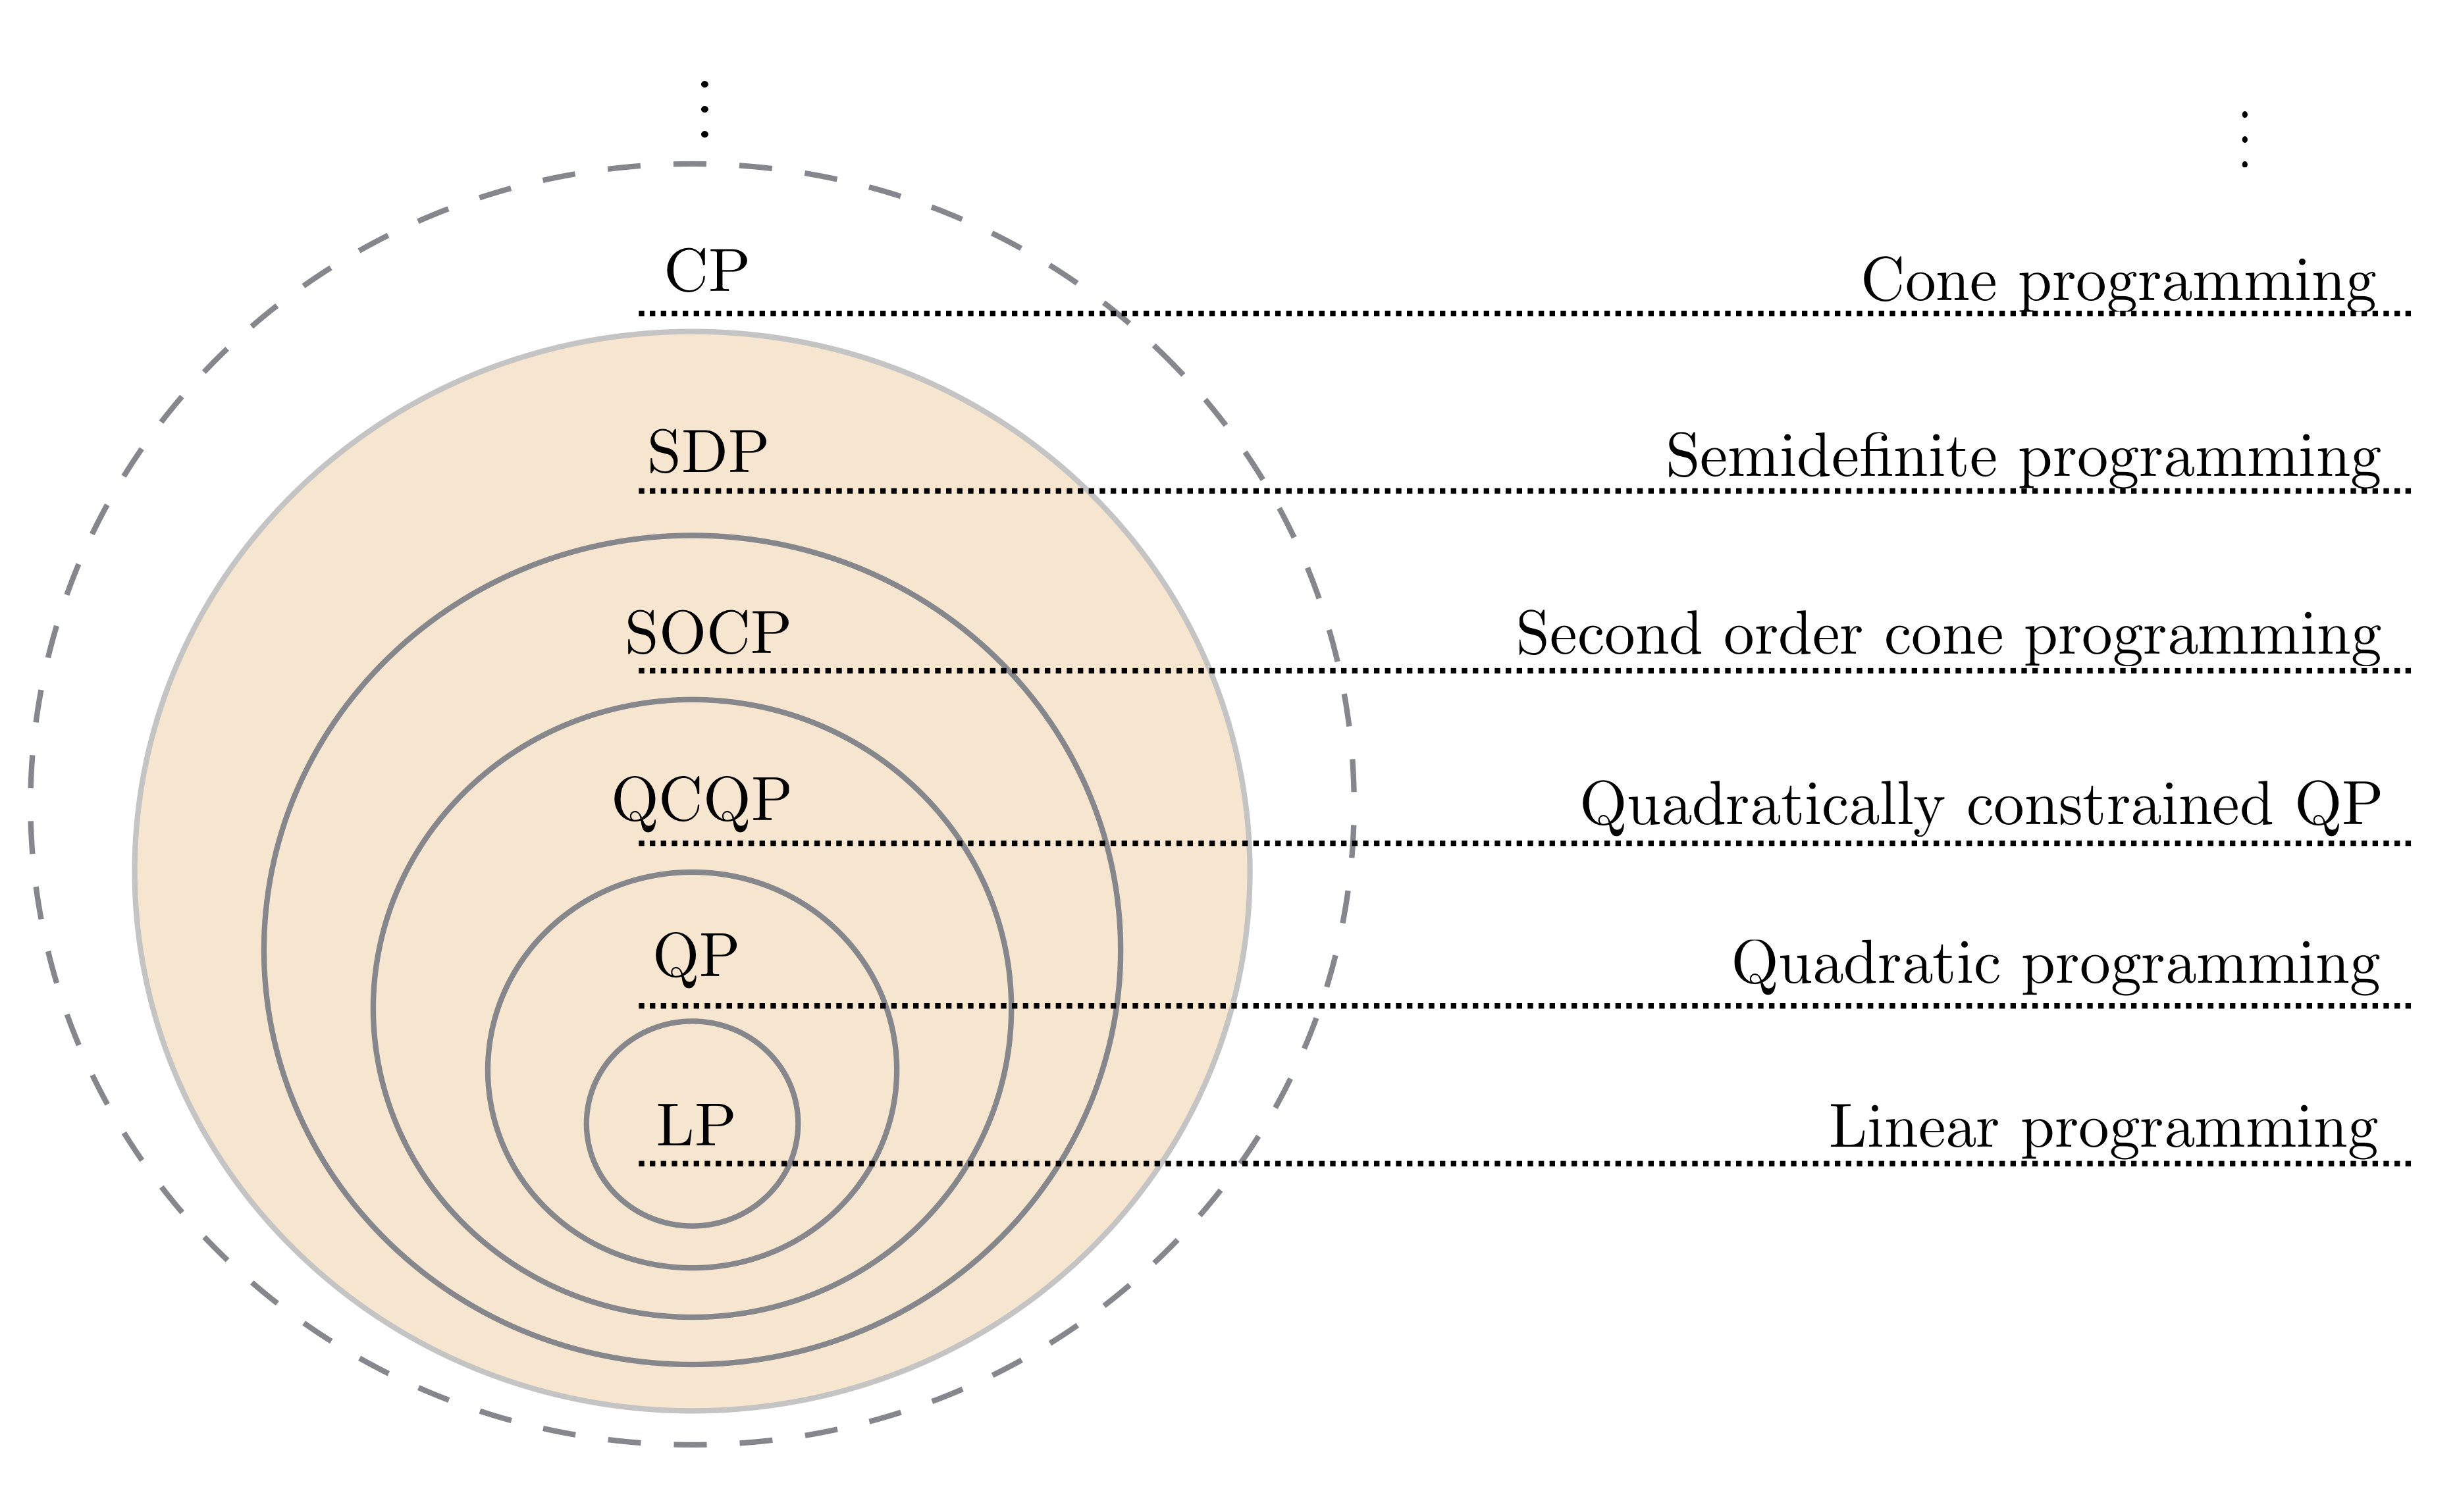
\includegraphics[width=12cm]{classification.jpeg}
    \caption{The hierarchy of disciplined convex optimization~\cite{classification}}\label{f:classification}
    \end{center}
\end{figure}

\subsection{Task 01}

In general, a SDP can be described in the following form: 

\begin{equation}
\begin{aligned}
\min_{} \quad & C\cdot X\\
\textrm{s.t.} \quad & A_j \cdot X = b_j , j \in [m], \; X,A_1,...,A_m \in \mathbb{R}^{n\times n}, \; b_1,...,b_m\in \mathbb{R}\\
  & X \succeq 0,\\
\end{aligned}
\end{equation} where both $X$ and $C$ be symmetric matrices. Consider the following example:
\begin{equation}
    A_1 = \begin{bmatrix}
1 & 0 & 1\\ 
0 & 3 & 7\\ 
1 & 7 & 5
\end{bmatrix}, \; A_2 = \begin{bmatrix}
0 & 2 & 8\\ 
2 & 6 & 0\\ 
8 & 0 & 4
\end{bmatrix}, \; C = \begin{bmatrix}
1 & 2 &3 \\ 
2 & 9 & 0\\ 
3 & 0 &7 
\end{bmatrix}, \; b_1=11, b_2 = 19
\end{equation}

\begin{enumerate}
    \item Can you guess the values of n and m? 
    \item How many parameters to be optimized in this particular case? 
    \item Prove that $C \cdot X = x_{11} + 4x_{12} + 6x_{13} + 9x_{22} + 0x_{23} + 7x_{33}$
    \item Assume $x_{ij}$ denotes the elements of X and constraints are given by $x_{11} + 2x_{13} + 3x_{22} + 14x_{23} +5x_{33} = 11$ and $4x_{12}+16x_{13}+6x_{22}+4x_{33} = 19$. Aside this general case, what can you say about when all the entries of $A_j$ and $X$ become zeros except diagonal entries?
\end{enumerate}

\subsection{Task 02}
A ellipsoid in $\mathbf{R}^n$ has the following form
\begin{equation}\label{ellipsoid}
    Ellipsoid = \{x | (x-x_c)^TP^{-1}(x-x_c) \leq 1\} = \{x_c+Ax|\left \|x \right \|_2 \leq 1 \}, \; P=P^T \succ 0
\end{equation} where A is square and nonsingular ($A=P^{1/2}$). The matrix P determines the how far the ellipsoid extends in every direction from $x_c$ whose length is determined by $\sqrt{\lambda_i}$, where $\lambda_i$ is the $i^{th}$ eiegen value. As given in (\ref{ellipsoid}), ellipsoid can be formulated in different ways, 

% https://math.stackexchange.com/questions/1402910/why-is-a-positive-definite-matrix-needed-in-the-ellipsoid-matrix-representation
% positive definite matrix P = U^TU where U is invartible, P = V B V^-1 
% http://www.wisdom.weizmann.ac.il/~robi/teaching/AdvAlgs2008/handout7.pdf

\begin{equation}\label{ellipsoid1}
    Ellipsoid = \varepsilon  = \{x | (x-x_c)^TP^{-1}(x-x_c) = \{x | (x-x_c)^TE(x-x_c)  \leq 1\}
\end{equation}
Intuition is to check given points $x_i$ whether inside or outside of (\ref{ellipsoid1}). In other words, the following condition must be satisfied
\begin{equation}\label{ellipsoid1}
   (x_i-x_c)^TE(x_i-x_c) \leq 1, \quad i=1,...,m
\end{equation} Hence, finding a optimal vector $x_c\in \mathbb{R}^n$ and positive definite symmetric matrix E which minimizes the volume subject to \ref{ellipsoid1}. The volume of an ellipsoid can be determined by\cite{Moshtagh_minimumvolume} 
\begin{equation}
     Vol(\varepsilon) = \frac{v_0}{\sqrt{det(E)}} = v_0 det(E^{-1})^{1/2},
\end{equation} where $v_0$ is the volume of the unit hypersphere in $\mathbb{R}^{n}$. Thus, minimizing the volume (or $det(E^{-1})^{1/2}$) can be formulated as an optimization problem as follows:

\begin{equation}\label{find_volume}
\begin{aligned}
\min_{E,c} \quad & det(E^{-1})^{1/2}\\
\textrm{s.t.} \quad & (x_i -x_c)^TE(x_i-x_c) \leq 1 \; i=1,...,m\\
  & E \succeq 0\\
\end{aligned}
\end{equation}

Can we solve this as convex optimization problem? If not how can we solve this? By change of variables, (\ref{ellipsoid1}) can be reformulated as follows:
\begin{equation}
    \varepsilon = \{ x \in \mathbb{R}^n \; | \; \left \| Ax-b \right \|_2 \leq 1\}
\end{equation} where $A = E^{1/2}$ and $b = E^{1/2}x_c$. Thus, (\ref{find_volume}) can be rewritten as:

\begin{equation}\label{find_volume}
\begin{aligned}
\min_{A,b} \quad & -log det(A)\\
\textrm{s.t.} \quad & \left \| Ax-b \right \|_2 \leq 1 \; i=1,...,m\\
  & A \succeq 0\\
\end{aligned}
\end{equation} where norm constraints $\left \| Ax-b \right \|_2 \leq 1 $, which are convex inequalities, can be expressed as Linear Matrix Inequalities (LMIs). 
\begin{equation}
    \left \| Ax-b \right \|_2 \leq 1  = \begin{bmatrix}
I & Ax_i-b\\ 
 (Ax_i-b)^T & I 
\end{bmatrix} \geq 0
\end{equation}

Where does this log comes form and what the reasoning behind this? When minimizing the $det(A^{-1})$, it might be fail due to non-convex nature. By applying log transformation the problem (\ref{find_volume}) guarantee to be strictly convex. This can be solved using any convex optimization solver. The following code can be used to design the problem in CVXPY,

% \begin{minted}
% [frame=lines, framesep=2mm, baselinestretch=1.2,]
% {python}
% A = cp.Variable((dim,dim), PSD=True)
% b = cp.Variable(dim)      
% constraints = [cp.norm(A@X[i]-b,2)<= 1 for i in range(len(X))]
% prob = cp.Problem(cp.Minimize(-cp.log_det(A)), constraints)
% optval = prob.solve()
% \end{minted}

\subsection{Task 03} 
How can you estimate the maximum volume that encloses an inscribed ellipsoid of convex hull?
Let's say you are given a set of inequalities that describes by a polytope:

\begin{equation}
    P = \{ x \in \mathbb{R}^n \; a_i^Tx \leq b_i, \; i=1,...,m\}
\end{equation} So intention is to find inscribed ellipsoid with maximum volume. Let $\varepsilon$ be the ellipsoid that is to be estimated: 
\begin{equation}
    \varepsilon = \{x \; | \; x = By + d, y \in \mathbb{R}^n, \left \| y \right \|_2 \leq 1, \; B= B^T \succ 0\}.
\end{equation} In order to maximize the volume, the condition $\varepsilon \subseteq P$ should be satisfied; this condition can be formed as the following way as a set of inequalities:
\begin{equation}
  \left \| Ba_i \right \| + a_i^Td \leq b_i, \; i=0,...,m
\end{equation}

Now we are ready to find the inscribed ellipsoid. 
\begin{equation}\label{max_volume}
\begin{aligned}
\min_{B,d} \quad & -log det(B)\\
\textrm{s.t.} \quad &\left \| Ba_i \right \| + a_i^Td \leq b_i, \; i=0,...,m \\
  & B \succeq 0\\
\end{aligned}
\end{equation} 


% \begin{minted}
% [frame=lines, framesep=2mm, baselinestretch=1.2,]
% {python}
% B = cp.Variable((dim,dim), PSD=True)
% d = cp.Variable(dim)
% constraints = [cp.norm(B@A[i],2)+A[i]@d<=b[i] for i in range(len(A))]
% prob = cp.Problem(cp.Minimize(-cp.log_det(B)), constraints)
% optval = prob.solve()
% \end{minted}


\begin{figure}[H]
    \begin{center}
    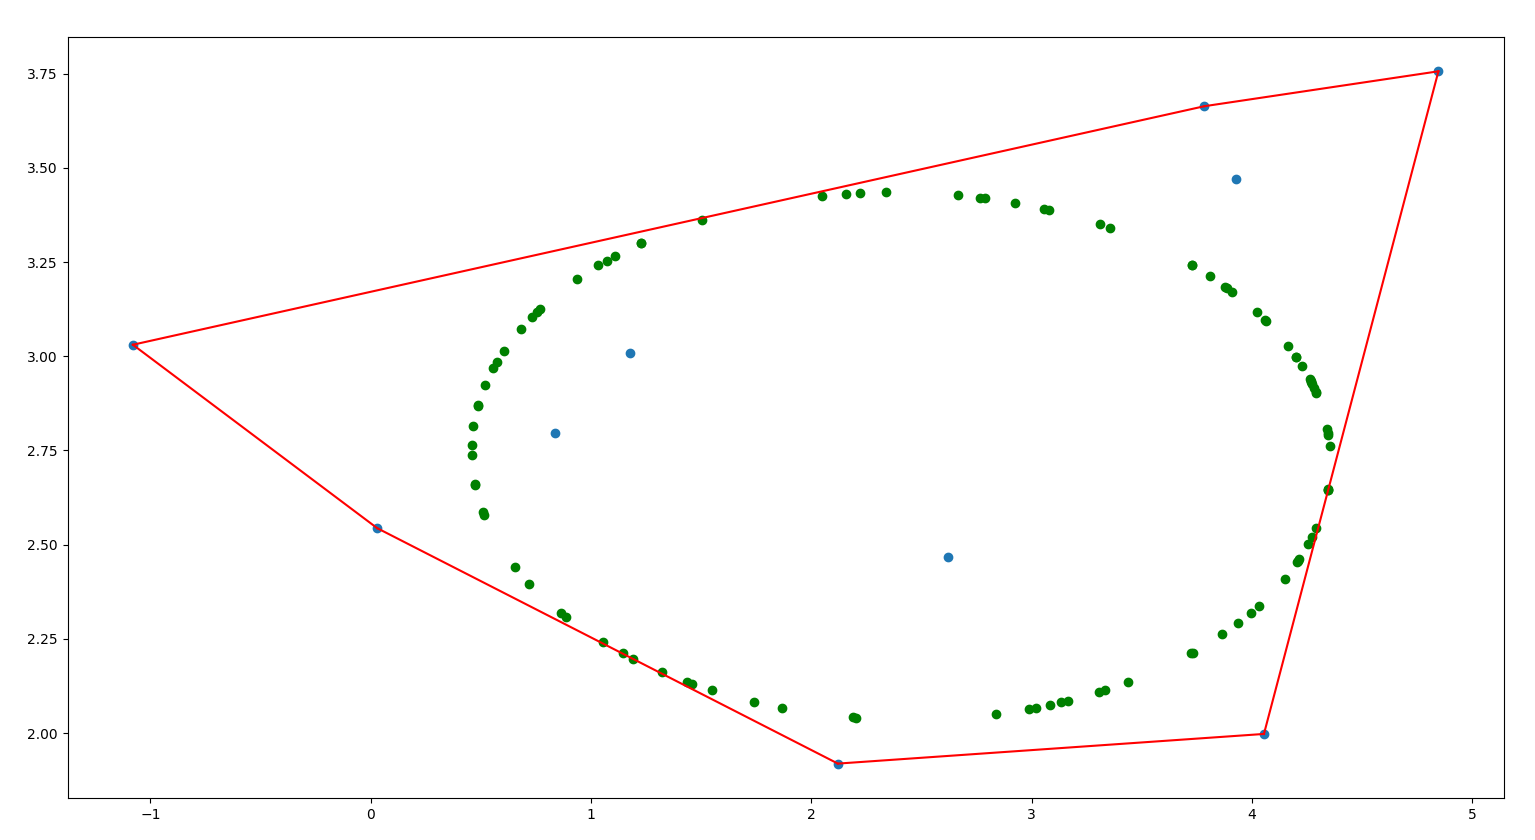
\includegraphics[width=12cm]{min_volume.png}
    \caption{Maximum volume that encloses an inscribed ellipsoid of convex hull}\label{f:min_volume}
    \end{center}
\end{figure}

\printbibliography
\end{document}